\chapter{Simplicial localization}

\begin{refsection}

The goal of this paper is to present the simplicial localization as defined by Dwyer ad Kan in their articles \cite{dksimplicial}, \cite{dkcomputing} and \cite{dkfunction}. The reader is supposed to know the theory of model category and homotopy category.

\begin{flushright}
Brice Le Grignou
\end{flushright}

\section{Introduction}

\subsection{Localization and higher homotopy}

Let $M$ be a model category. The axioms of model categories imply more than just homotopy relations. For example, one can describe homotopy relations between homotopy relations (see \cite[2.3]{fromHAtoHAG}). The homotopy localization loose this hidden data as it merges maps which are joined by an homotopy relation. We try here to describe this "higher homotopy structure".\\

We present first the homotopy function complexes and their relations with homotopy. Then we present the two Dwyer-Kan localizations which is the core of the paper. Finally a small theorem states that the two approach give us the same homotopy.

\subsection{Notations and terminology}

\begin{enumerate}
\item If $C$ is a category and $X,Y \in Obj(C)$, then $C(X,Y)$ denotes the set of morphisms from $X$ to $Y$ in $C$
\item If $C$ is a category, then $sC$ is the category of simplicial objects over $C$ 
\item All the categories are small (except when specified). We do not deal of set theory or universes theory issues. This is motivated by the following theorem.
\item Simplicial categories: the usual definition of a simplicial category is an enrichment over the category of simplicial set. As the categories are supposed small, one can use the following presentation:
\begin{enumerate}
\item If $A$ is a simplicial category (with small set of objects); then let $A-cat$ the category whom objects are (small) categories with $Obj(A)$ as set of objects and whom morphisms are functors which sends an object to itself.
\item Then $A$ is nothing but a simplicial object over the category $A-cat$
\end{enumerate}
\item A weak equivalence of simplicial categories $S :A \rightarrow B$ is a functor of simplicial categories such that
\begin{enumerate}
\item If $\pi_0 A$ is the category with the same objects as $A$ and such that $(\pi_0 A) (X,Y)= \pi_0 (A(X,Y))$ then $S$ induces an equivalence of (ordinary) categories $\pi_0 A \simeq \pi_0 B$ ($\pi_0 B$ is defined in the same way)
\item $A(X,Y) \rightarrow B(SX,SY)$ is a weak homotopy equivalence.
\end{enumerate}
\item In the previous definition, if $S$ is nothing but a morphism in $sA-cat$, then only the second point holds.
\item In a model category we represent the cofrations and the the fibrations by respectively: $\xymatrix{{} \ar@{^{(}->}[r] & {}}$ and $\xymatrix{{} \ar@{->>}[r] & {}}$. The weak equivalences are noted with a $\sim$.
\end{enumerate}

\begin{thm}[{\cite[Thm. 2.3]{dkfunction}}]
Let $A$ a simplicial category, and $B \in A$ a small simplicial subcategory. Then there exists a small simplicial subcategory $B'$ such that $B \subseteq B' \subseteq A$ and $B'(X,Y) \rightarrow A(X,Y)$ is a weak homotopy equivalence for all $X,Y \in B'$
\end{thm}

\section{Motivation of the simplicial localization}

\subsection{Simplicial model categories}

\begin{defin}
A simplicial model category $M$ is a model category which is also a simplicial category; this means equivalently:
\begin{enumerate}
\item $M$ is a simplicial enriched category, such as we have distinguished three classes of elements of the sets $Map(X,Y)$
\item $M$ is an element of $sM-cat$ such as $M_0$ has a model structure
\end{enumerate}
Furthermore, $M$ respects the following axioms:
\begin{enumerate}
\item For every two objects $X, Y$ of $M$, and every simplicial set $K$, there exists two objects $X\otimes K$ and $Y^K$ of $M$ such that we have isomorphisms of simplicial sets:
\begin{equation}
Map(X\otimes K, Y) \simeq Map_{sSet}(K, Map(X,Y)) \simeq Map(X, Y^K)
\end{equation}
\item If $i: A\rightarrow B$ is a cofibration in $M$ and $p:X \rightarrow Y$ is a fibration, then:
\begin{equation}
Map(B,X) \rightarrow Map(A,X) \times_{Map(A,Y)} Map(B,Y)
\end{equation}
is a fibration which is acyclic if either $i$ or $p$ is acyclic.
\end{enumerate}
\end{defin}

The simplicial model category is close to the ideal concept we want to approach from a simple model category in order to get the "higher order information" which is contained in the mapping spaces. We will see how this property happens.

\subsection{Homotopy function complexes}

Let $M$ be a model category, and $W$ a the subcategory of weak equivalence.

\begin{defin}
Let $Y$ an object of $M$. A simplicial resolution of $Y$ is a simplicial object over $M$ noted $Y_*$ together with a weak equivalence $Y \rightarrow Y_0$ such that
\begin{enumerate}
\item the object $Y_0$ is fibrant
\item all faces maps in $Y_*$ are acyclic fibrations. Hence, all the objects $Y_n$ are fibrants.
\item Let $(d_*, Y_n)$ the diagram:
\begin{enumerate}
\item for every $0 \le i \le n+1$, a copy $(d_i; Y_n)$ of $Y_n$
\item for every $0 \le i < j \le n+1$, a copy $(d_id_j,Y_{n-1})$ of $Y_{n-1}$
\item pair of maps: $(d_j, Y_n) \rightarrow (d_id_j,Y_{n-1}) \leftarrow (d_j, Y_n)$. These arrows are acyclic fibrations. 
\end{enumerate}
Then the map $Y_{n+1} \rightarrow (d_*,Y_n)$ is a fibration.
\end{enumerate}
\end{defin}

\begin{defin}
A simplicial resolution $Y_*$ of $Y$ can be viewed as a simplicial object over $M$ together with a simplicial map $i:Y \rightarrow Y_*$ (here $Y$ represents the constant simplicial object over $M$ made from the object $Y$), and having some further properties. Then one can define a map of simplicial resolutions of $Y$, $f:Y_* \rightarrow {Y'}_*$ as a simplicial map which makes the following diagram commute:
\[ \xymatrix{Y \ar[rr] \ar[dr] && {Y'_*} \\ & Y \ar[ur]} \]
\end{defin}


\begin{defin}
The notion of cosimplicial resolution and map between cosimplicial resolutions are defined dually from the notion of simplicial resolution and map of simplicial resolutions.
\end{defin}

With these notions, one can try to state the definition:

\begin{defin}
$M(X^*,Y_*)$ has an obvious structure of bisimplicial set for $X^*$ a cosimplicial resolution of $X$ and $Y_*$ a simplicial resolution of $Y$. The homotopy complex of $(X,Y)$ is then defined as $diag M(X^*,Y_*)$ .
\end{defin}

However, one needs some machinery to make this definitions coherent. Indeed one has to check that the homotopy can be defined for two objects $(X,Y)$ and that it does not depens on the resolutions chosed. The first requirement is answered by: 

\begin{prop}
Every object of a model category $M$ has simplicial and a cosimplicial resolutions.
\end{prop}

\begin{proof}
Let's show the result by induction for a simplicial resolution. One adds a requirement of this simplicial resolution (usefull for the construction): the degeneracies are acyclic cofibrations.
\begin{itemize}
\item If $*$ is the final object of $M$, then $Y \rightarrow *$ can be factorized through : $\xymatrix{{Y} \ar@{^{(}->}[r]^{\sim} & {Y_0} \ar@{->>}[r] & {*}}$. Then one got the fibrant element $Y_0$ and an acyclic fibration from $Y$ to $Y_0$.
\item If one has the elements $Y_i$ for $0 \leq i \leq n$ with the corresponding faces and degeneracies maps which are respectively acyclic fibrations and acyclic cofibrations, then one defines $(s_*,Y_n)$ as the direct limits of the diagram made of copies $(s_i,Y_n)$ of $Y_n$ for $0 \leq i \leq n$ and copies $(s_i s_j, Y_{n-1})$ of $Y_{n-1}$ for $0 \leq i < j \leq n$ together with maps $\xymatrix{{(s_i,Y_n)}  & {(s_i s_j, Y_{n-1})} \ar@{^{(}->}[l]^{s_{j-1}} \ar@{^{(}->}[r]^{s_{i}} & {(s_j,Y_n)}}$. Then one has easily a weak equivalences $\xymatrix{{(s_*,Y_n)} \ar[r]^{\sim} & {(d_*,Y_n)}}$ which can be factorized through $\xymatrix{{(s_*,Y_n)} \ar@{^{(}->}[r]^{\sim} &{Y{n+1}} \ar@{->>}[r]^{\sim} & {(d_*,Y_n)}}$.
\end{itemize}
The cosimplicial resolution is created dually.
\end{proof}


\begin{rmk}
In the proof we had added a property: the map $Y \rightarrow Y_0$ and the degeneracies are acyclic cofibrations. Such a simplicial resolution is called cofibrant. We define dually the notion of fibrant cosimplicial resolution. The proof of the previous property shows that every object of $M$ has cofibrant simplicial resolutions and fibrant cosimplicial resolutions.
\end{rmk}

The next lemma uses this last notion to make links between the various homotopy function complexes one can construct.

\begin{lemma}[{\cite[6.9 and 6.10]{dkfunction}}]
\begin{enumerate}
\item Let $Y_*$ and $Y'_*$ be simplicial resolutions of $Y$. Then, if $Y'_*$ is cofibrant, there exists a map of resolutions $Y_* \rightarrow Y'_*$.
\item Let $X^*$ and $X'^*$ be cosimplicial resolutions of $X$. Then, if $X'^*$ is fibrant, there exists a map of resolutions $X'^* \rightarrow X^*$
\end{enumerate}
\end{lemma}

\begin{proof}[Sketch of proof.]
The maps are constructed by induction
\end{proof}

\begin{prop} $[4,17.3.4]$
If $f:{X'}^* \rightarrow X^*$ is a map of cosimplicial resolutions of $X$ and $g:Y_* \rightarrow {Y'}_*$ is a map of simplicial resolutions of $Y$, then they induced a map of simplicial set $diag M(X^*,Y_*) \rightarrow diag M({X'}^*,{Y'}_*)$ which is a weak homotopy equivalence
\end{prop}

\begin{cor}
One can find a finite string of weak homotopy equivalences between two homotopy function complexes constructed for the pair of objects $(X,Y)$. Hence, the homotopy function complex is unique up to weak homotopy equivalence.
\end{cor}

The next proposition allows us to link the homotopy function complexes to the usual notion of homotopy in a model category:

\begin{prop}
\begin{enumerate}
\item If $X^*$ is cosimplicial resolution in $M$, then $X^0 \sqcup X^0 \rightarrow X^1 \rightarrow X^0$ is a cylinder object of $X^0$.
\item If $Y_*$ is simplicial resolution in $M$, then $Y_0 \rightarrow Y_1 \rightarrow Y_0 \times Y_0$ is a path object of $Y_0$.
\end{enumerate}
\end{prop}

Then, a cosimplicial resolution of $X$ is a sort of "higher cylinder objects" collection for a cofibrant approxiation of $X$. Dually, a simplicial resolution of $Y$ is a sort of "higher path objects" collection for a fibrant approximation of $Y$.


\subsection{Homotopy function complexes and simplicial model categories}

Let $M$ be a simplicial model category

\begin{prop}
\begin{enumerate}
\item If $X$ is an object of $M$ and $X'$ is a cofibrant approximation of $X$, then the cosimplicial object defined by $X^n = X' \otimes \Delta^n$ is a cosimplicial resolution of $X$
\item If $Y'$ is a cofibrant approximation of $Y \in M$, then the simplicial object defined by $Y_n = Y'^{\Delta^n}$ is a simplicial resolution of $Y$
\end{enumerate}
\end{prop}

\begin{cor}
If $X$ is cofibrant and $Y$ is fibrant, then the homotopy function complex of $(X,Y)$ is $Map(X,Y)$.
\end{cor}

\subsection{Homotopical limit}

This is an other way to define a "mapping space" between two objects in a model category.\\

We start with the definition of homotopy limits:

\begin{defin}
If $I$ is a (small) indexing category, then define $C^I$ the category of functors $I \rightarrow C$. Then let $W_I$ the subcategory of $C^I$ spaned with the morphisms of functors (natural transformations) which are objectwise in $W$. Then, the constant functor $C \rightarrow C^I$ leads to a functor $C \rightarrow C^I[(W_I)^{-1}]$ which can be factorized through:
\begin{equation}
c: C[W^{-1}] \rightarrow C^I[(W_I)^{-1}]
\end{equation}
\begin{enumerate}
\item the homotopy limit of $A \in obj(C^I[(W_I)^{-1}])$ is (if it exists) the object $holim_I(A)$ of $C[W^{-1}]$ such that we have a isomorphism of functors (in $B$) $Hom_{C[W^{-1}]}(holim_I(A),B) \simeq Hom_{C^I[(W_I)^{-1}]}(A, c(B))$. The functoriality in $A$ of the previous isomorphism makes us define the holimit functor (if it exists) as a left adjoint of $c$
\item The hocolimit functor is a right adjoint of $c$ (if such a functor exists).
\end{enumerate}
\end{defin}

\begin{rmk}
The $holim$ and $hocolim$ are introduced because the usual $lim$ and $colim$ in $C$ is not localized in a good way. 
\end{rmk}

\begin{defin}
If $Y$ is an object of $C$, then:
\begin{enumerate}
\item If we consider the object $Y^K=holim(\Delta \rightarrow : [n] \mapsto \prod_{K_n} Y)$, this definition induces a functor $Ho(sSet) \rightarrow C[W^{-1}] : K \mapsto Y^K$.
\item Then a functor $Map : Ho(sSet) \rightarrow Set : K \mapsto Hom(X,Y^K)$.
\item The mapping space is a simplicial set which represents the functor.

\end{enumerate}
\end{defin}


\section{Two definitions of the simplicial localization}

For the two first parts of this section, we don't need a model structure on the category but just a category $C$ with a subcategory $W$. The aim is to understand the localization of $C$ with respect to $W$ through simplicial categories.

\subsection{Standard simplicial localization}

\subsubsection{Free categories}

Here we develop the machinery which permits to define the standard simplicial localization of a category.

\begin{defin}
A free category $C$ is a category such that there is a set of non-identity maps $S$ such that every map in $C$ is written in a unique way as a finite composition of maps of $S$ . If such $S$ exists, then it is unique. The elements of $S$ are called the generators of $C$.
\end{defin}


\begin{defin}
If $C$ is a category, the category $FC$ is the free category which has as generators the set of non-identity maps. In other words, $FC$ is such that:
\begin{itemize}
\item $Obj(FC)=Obj(C)$
\item the morphisms of $FC$ are the trees of heigh 1 with non-identity maps of $C$ as leaves, and such that these leaves can be composed (in the picture it means that one can compose $a \circ b \circ c$):\\
\begin{center}
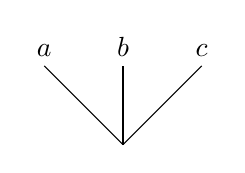
\begin{tikzpicture}
\draw (1,0) -- (0,1) node[above]{$a$} ;
\draw (1,0) -- (1,1) node[above]{$b$} ;
\draw (1,0) -- (2,1) node[above]{$c$} ;
\end{tikzpicture}
\end{center}
Of course, the source of such a map is the source of the first leave and the target is the target of the last leave. The identity maps are represented by the empty trees and the composition consists in joining the roots.
\end{itemize}
\end{defin}

One can repeat the process several times: $F^kC$ is the category with the same objects as $C$ and, as morphisms, the trees of heigh $k$ with maps of $C$ as leaves, which can be composed. The composition consists in joining the roots.\\

There is an obvious functor $\phi$ from $FC$ to $C$: it sends an object to itself ($Obj(FC)=Obj(C)$), and a tree (ie a morphism) to the composition of its leaves (in the previous tree picture, it sends the tree to $a \circ b \circ c$). Define also the obvious functor $:C \rightarrow FC$ which sends an object to itself and a morphism $a$ to the corresponding generator in $FC$, ie:
\begin{center}
\begin{tikzpicture}
\draw (0,0) -- (0,1) node[above]{$a$} ;
\end{tikzpicture}
\end{center}  


Similarly, there are natural functors between $F^2C$ and $FC$; one functor from $F2C$ to $F^2C$ and two functors in the opposite sense:
\begin{itemize}
\item $\phi F: F^2C \rightarrow FC$ reduces the branches between the height 1 and 2, ie:
\begin{center}
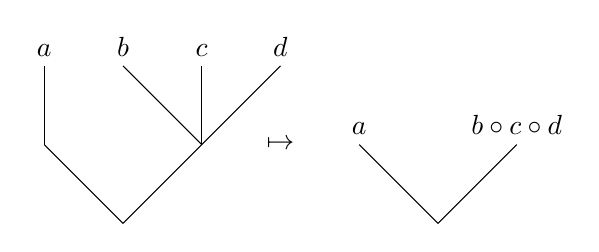
\begin{tikzpicture}
\draw (1,0) -- (0,1) ;
\draw (0,1) -- (0,2) node[above]{$a$} ;
\draw (1,0) -- (2,1) ;
\draw (2,1) -- (1,2) node[above]{$b$} ;
\draw (2,1) -- (2,2) node[above]{$c$} ;
\draw (2,1) -- (3,2) node[above]{$d$} ;

\draw (3,1) node{$\mapsto$};

\draw (5,0) -- (4,1) node[above]{$a$} ; 
\draw (5,0) -- (6,1) node[above]{$b \circ c \circ d$} ;
 
\end{tikzpicture}
\end{center}  
\item $F\phi : F^2C \rightarrow FC$ reduces the branches between the height 0 and 1, ie:

\begin{center}
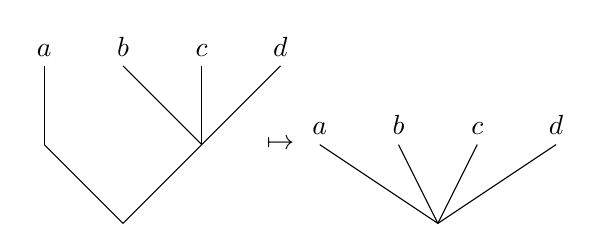
\begin{tikzpicture}
\draw (1,0) -- (0,1) ;
\draw (0,1) -- (0,2) node[above]{$a$} ;
\draw (1,0) -- (2,1) ;
\draw (2,1) -- (1,2) node[above]{$b$} ;
\draw (2,1) -- (2,2) node[above]{$c$} ;
\draw (2,1) -- (3,2) node[above]{$d$} ;

\draw (3,1) node{$\mapsto$};

\draw (5,0) -- (3.5,1) node[above]{$a$} ; 
\draw (5,0) -- (4.5,1) node[above]{$b$} ;
\draw (5,0) -- (5.5,1) node[above]{$c$} ;
\draw (5,0) -- (6.5,1) node[above]{$d$} ;
 
\end{tikzpicture}
\end{center}

\item Define also $\psi :: FC \rightarrow F^2C$:
%\begin{comment}
\begin{center}
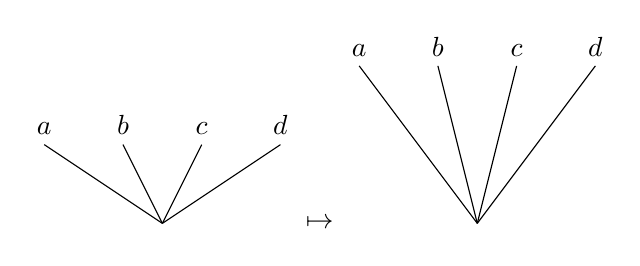
\begin{tikzpicture}
\draw (1.5,0) -- (0,1) node[above]{$a$} ; 
\draw (1.5,0) -- (1,1) node[above]{$b$} ;
\draw (1.5,0) -- (2,1) node[above]{$c$} ;
\draw (1.5,0) -- (3,1) node[above]{$d$} ;

\draw (3.5,0) node{$\mapsto$};

\draw (5.5,0) -- (4,2) node[above]{$a$} ; 
\draw (5.5,0) -- (5,2) node[above]{$b$} ;
\draw (5.5,0) -- (6,2) node[above]{$c$} ;
\draw (5.5,0) -- (7,2) node[above]{$d$} ;
\end{tikzpicture}
\end{center}
%\end{comment}
\end{itemize}

One notices for instance that $(F \phi) \psi=(F \phi) \psi$. One can also continue the process to higher order of free category; one then define in the same way $n$ functors from $F^n C$ to $F^{n-1} C$ and $n$ functors 

\begin{prop}
$(F^{k+1}C)_k$ together with the functors defined above is a simplicial category.
\end{prop} 

Furthermore this new category has the same homotopy type as $C$ (if we consider as a constant simplicial category

\begin{prop}
$(F^{k+1}C)_k \rightarrow C$ (functor unduced by the reduction of the trees) is a weak equivalence of categories (that means that it induces weak equivalences on the simplicial morphisms sets).
\end{prop} 

\begin{proof}[Sketch of the proof.]
Every tree of height $k$ is equivalent (in the homotopy sense) to the tree of same height and with only one leave which is the composition of the leaves.
\end{proof}

\subsubsection{The localization: definitions and first properties}

Along those lines, the morphisms of the localized categories $C[w^{-1}]$ are the tree of height $1$ such that its leaves are a succession of maps of $C$ and of $W$ (quotiented through an equivalence relation). The underlying idea of the standard simplicial localization is to look at the localization of $F^{k} C$ by $F^{k} W$.\\

Then, with few changes in the way of thinking with the respect to what we have in the previous sub-part, one can define: 

\begin{defin}
The (standard) simplicial localization of $(C,W)$ is the simplicial category $L(C,W)$ defined by:
\begin{equation}
L(C,W)_n=F^{n+1}C[(F^{n+1}W)^{-1}]
\end{equation}
\end{defin}

The homotopy groups of this localization is expected to encode the higher homotopy data data of $C$ with respect to $W$. Actually the homotopy relations are basically generated by the relation of two trees which have the same dimension and can be constructed from one same bigger tree. In dimension $0$, it gives the relation: 

\begin{prop}
$\pi_0 (LC(X,Y))=C[W^{-1}](X,Y)$
\end{prop}

\subsubsection{Generalization to simplicial categories}

One can generalise the notion of standard simplicial localization to simplicial categories.

\begin{defin}
If $A$ is a simplicial category, and $V$ a simplicial subcategory. The standard simplicial localization of $A$ with respect to $V$ is the simplicial category:
\begin{equation}
L(A,V)=diag(F^{*+1}A[(F^{*+1}V)^{-1}])
\end{equation} 
\end{defin}

We have something which is close of the old localization of an ordinary category if we take the path-components:
\begin{prop}
$\pi_0 (LB) =(\pi_0 B)[(im \pi_0 V)^{-1}]$
\end{prop}

Finally, let's see one lemma which can be useful:

\begin{lemma}[{\cite[6.3]{dksimplicial}}]
Let $A$ and $B$ two simplicial $C$-categories, $U$ a simplicial subcategory of $A$ and $V$ a simplicial subcategory of $B$, $S: A \rightarrow B$ a functor such that $S(U) \subset V$, and such that $S: A \rightarrow B$ and $S: U \rightarrow V$ are weak equivalence. Then the induced map $LA \rightarrow LB$ is a weak equivalence.
\end{lemma}

The demonstration of this last lemma is more complicated. One needs some machinery, as for instance a model structure on the category of the simplicial categories with the same objects as $C$ (this last category is not small).


\subsection{Hammock localization}

\subsubsection{Definition and first properties}
Let $C$ be a (small) category an $W$ a subcategory. Let's define the simplicial set $L^H (C,W)(X,Y)$ (or shortly $L^H C(X,Y)$); the $k$-simplices are the "reduced hammocks" of width $k$ and any length between $X$ and $Y$:

\[
\xymatrix{& {C_{0,0}} \ar@{-}[r] \ar[d] & {C_{0,1}} \ar[d] \ar@{--}[r] & {C_{0,n-1}} \ar@{-}[d] \ar@{-}[ddr] \\
& {C_{1,0}} \ar@{-}[r] \ar[d] & {C_{1,1}} \ar@{-->}[ddd] \ar@{--}[r] & {C_{1,n-1}} \ar@{-->}[ddd] \ar@{-}[dr] \\
X \ar@{-}[uur] \ar@{-}[ur] \ar@{--}[r] \ar@{-}[ddr] & {C_{2,0}} \ar@{-->}[dd] &&& {Y} \\
                                                                             \\
& {C_{k,0}} \ar@{-}[r] & {C_{k,1}} \ar@{--}[r] & {C_{k,n-1}} \ar@{-}[uur]}
\]

such that:
\begin{enumerate}
\item $n$, the length is $\geq 0$ (if $n=0$, the hammock consists in $k$-times the same morphism from $X$ to $Y$).
\item all vertical maps are in $W$.
\item in each column, all maps go to the same direction and if they go to the left, then they are in $W$.
\item the maps in adjacent columns go in different directions.
\item no column contains only identity maps.
\end{enumerate}

The $i^{th}$ face map $d_i$ consists in omitting the $i^{th}$ row. The $j^{th}$ degeneracy map consists in repeating the $j^{th}$ row. If the resulting hammock is not reduced (it can happen after the application of a face map), then one applies a reduction process:
\begin{enumerate}
\item if a column contains only identity maps, then one omits it.
\item one composes two adjacent columns whenever they go in the same direction
\end{enumerate}

Furthermore, there exists a distinguished vertices $id \in L^HC(X,X)$; if $X,Y$ and $Z$ are object of $C$, then one can also composition law $L^HC(X,Y) \times L^HC(Y,Z) \rightarrow L^H C(X,Z)$ which consists in, in each dimension, compose the hammocks and then reduce the resulting hammock. Then:

\begin{prop}
$L^H (C,W)$ is a simplicial category.
\end{prop}

The morphisms from $X$ to $Y$ of the localized category $C[W^{-1}]$ are the strings of successive arrows (i.e the elements of $L^HC(X,Y)_0$) quotiented by an equivalence relation. This equivalence is generated by the relation I call $\Re$; if $f,g \in L^HC(X,Y)_0$ then $ f \Re g$ if and only if:

\begin{center}
$\exists h \in L^H C(X,Y)_1 , d_0 (h)=f , d_1 (h)=g$
\end{center}

This just means:

\begin{prop}
For two objects $X,Y \in C$, then:
\begin{equation}
\pi_0 (L^H C(X,Y))=C[W^{-1}](X,Y)
\end{equation}
\end{prop}

Therefore, the underlying idea of the hammock localization is to study in a simplicial set the homotopy of string of arrows. Applying the equivalence gives us the usual localization, but makes us loose the higher homotopy data. The hammock localization is the good object to study this higher homotopy data.


\subsubsection{Generalisation to simplicial categories and link with the standard simplicial localization}

One can generalize the hammock localization to simplicial categories; if $B$ is a simplicial category and $V$ a simplicial subcategory (i.e a subcategory of $B$ together with inclusions of simplicial sets $V(X,Y) \rightarrow B(X,Y)$ which commute with the definition of identity and the composition):
\begin{enumerate}
\item $L^H(B,V)$ is an obviously defined bisimplicial category
\item the hammock localization of $B$ with respect to $V$ is $diag L^H(B,V)$
\end{enumerate}

\begin{rmk}
In the above description, one can equivalently use the formalism of simplicial objects over the category of simplicial (small) categories or of bisimplicial enriched categories;
\end{rmk}

There is an important lemma which comes with the description of the hammock of a simplicial category:

\begin{lemma}[{\cite[2.4]{dkcomputing}}]
If $A, B \in sC-cat$ (with the same set objects; see the introduction), and $U \subset A$, $V \subset B$ are simplicial subcategories, if $S : A \rightarrow B$ is a morphism in $sC-cat$ such that $S(U) \subset V$, and if $S:A \rightarrow B$ and $S: U \rightarrow V$ are weak equivalences (of simplicial $C$-categories), then it induces a weak equivalence of $C$-simplicial categories $diag L^H A \rightarrow diag L^H B$
\end{lemma}

This lemma is hard to prove. However, it is the main key for the next proposition:

\begin{prop}
If $C$ is a category and $W$ a subcategory (ordinary categories), then the natural functors:
\begin{equation}
L^H C \leftarrow diag L^H F^{*+1} \rightarrow F^{*+1} [(F^{*+1}W)^{-1}]
\end{equation}
are weak homotopy equivalences (in $sC-cat$).
\end{prop}

\begin{proof}[Ideas in the proof]
We don't make the proof but give its ingredients:
\begin{itemize}
\item the diagonal argument of bisimplicial sets
\item the homotopy lemma just above
\item the comparison lemma: if a category (ordinary) $D$ is freely generated by subcategories $E$ and $W$, then $L^H C \rightarrow C[W^{-1}]$ is a weak equivalence.
\end{itemize}
\end{proof}

So, we have make the link between the standard simplicial localization and the hammock localization. They are homotopy equivalent. Then one uses more the hammock localization as its definition is simpler and because it is simpler to work with it as we will see.

\subsubsection{The $II$-indexing category and hammock graphs}

The $II$ category is defined by:
\begin{enumerate}
\item its objects are the pairs $(S,T)$ of ordered subsets of $\mathbb{N}^*$ ($\mathbb{N}-\{0\}$) such that $S \cup T= \{1,...,|S \cup T|\}$.
\item the morphisms $(S,T) \rightarrow (S',T')$ are the order preserving maps $f: S \cup T \rightarrow S' \cup T'$ such that $f(S) \subseteq S'$ and $f(T) \subseteq T'$
\end{enumerate}

Let $C$ be a category and $W$ a subcategory (ordinary categories).

\begin{defin}
\begin{enumerate}
\item The category of $C$-graphs is defined by:
\begin{enumerate}
\item A $C$-graph is a graph (with directed edges i.e arrows) which set of points is $Obj(C)$.
\item A morphism $G_1 \rightarrow G_2$ of $C$-graph is the data of maps $G_1(X,Y) \rightarrow G_2(X,Y)$ for all $X$ and $Y$, objects of $C$, and where $G_1(X,Y)$ is the set of arrows from $X$ to $Y$ in $G_1$ (idem for $G_2$).
\end{enumerate}
\item the category of $C$-graphs corresponds to the category of $C$-simplicial categories but without the identity mapas and compositions. Indeed, one has the forgetful functor $C-cat \rightarrow C-graph$.
\item A simplicial $C$-graph is a simplicial object over the category of $C$-graph (or equivalently a $C$-graph with simplicial sets of arrows).
\item One has also the forgetful functor $sC-cat \rightarrow sC-graph$.
\item Weak equivalences between simplicial $C$-graphs are just morphisms of simplicial graphs which induce weak homotopy equivalences on the simplicial mapping spaces of arrows between two objects of $C$. This definition is the analogue to the definition of weak equivalence between simplicial $C$-categories.  
\end{enumerate}
\end{defin}

We can define a natural functor $\lambda C : II \rightarrow sC-graph$:
\begin{itemize}
\item An element of $II$ is equivalent to a word made with the letters $C$ and $W^{-1}$ in the way that transform, for example $(\{1,2\},\{3\})$ into $W^{-1} C C$.
\item From such a word, one made a simplicial $C$-graph describe by:
\begin{enumerate}
\item The arrows from $X$ to $Y$ (objects of $C$) are the unreduced hammocks:
\item the length of the hammocks is the length of the word we call $n$
\item The $i^{th}$ column is made of left-directed arrows of $C$ if the $(n+1-i)^{th}$ is $C$
\item The $i^{th}$ column is made of right-directed arrows of $W$ if the $(n+1-i)^{th}$ is $W^{-1}$  
\item These hammocks are organized in a simplicial set through the width as in $L^H C$.
\end{enumerate}
\item All of this is done functorially (because one can reduce parts of the hammocks and add column with the identity. For instance an injection in $II$ leads to the addition of identity maps in the corresponding $C$-graph). Therefore we have created a $II$-diagram in the category $sC-graph$
\item This diagram has a direct limit $lim \lambda C$
\end{itemize}


\begin{prop}
The reduction maps $r_{(S,T)} : \lambda C (S,T) \rightarrow L^H C$ (it is a morphism of the category $sC-graph$) induces a map $lim \lambda C \rightarrow L^H C$ which is a isomorphism.
\end{prop}

So we can see the hammock localization as a limit of graphs with simpler hammocks (of a definite type).

\begin{rmk}
This theory of $II$-diagrams is useful to prove the lemma introduced just above and non proved. However, we won't apply it to this purpose.
\end{rmk}

\subsubsection{Homotopy calculi of fractions}

Let $C$ be a category and $W$ a subcategory (ordinary categories).

\begin{defin}
$(C,W)$ is said to admit:
\begin{enumerate}
\item a homotopy calculus of (two-sided) fractions if, for every pairs $i,j >0$ the obvious maps in $sC-graph$ (adding a column with only identity):
\begin{equation}
W^{-1}C^{i+j}W^{-1} \rightarrow W^{-1}C^iW^{-1}C^jW^{-1}
\end{equation}
and
\begin{equation}
W^{-1}W^{i+j}W^{-1} \rightarrow W^{-1}W^i W^{-1} W^j W^{-1}
\end{equation}
are both weak equivalences (we consider the words as graph as seen just before).
\item a homotopy calculus of left fractions if, for every pairs $i,j >0$ the obvious maps in $sC-graph$:
\begin{equation}
W^{-1}C^{i+j} \rightarrow W^{-1}C^iW^{-1}C^j
\end{equation}
and
\begin{equation}
W^{-1}W^{i+j} \rightarrow W^{-1}W^i W^{-1} W^j
\end{equation}
are both weak equivalences.
\item a homotopy calculus of right fractions is defined in an analogue way.
\end{enumerate}
\end{defin}

The usefulness of the previous definition is due to the following proposition:

\begin{prop}[{\cite[6.2]{dkcomputing}}]
\begin{enumerate}
\item If $(C,W)$ admits a homotopy calculus of (two-sided) fractions, then the reduction maps
\begin{equation}
W^{-1}CW^{-1} \rightarrow L^H (C,W), W^{-1}WW^{-1} \rightarrow L^H (W,W)
\end{equation}
are weak equivalences.
\item one has the same kind of statement for the homotopy calculus of left or right fractions.
\end{enumerate}
\end{prop}

So, if the category admits a homotopy calculus of fractions, then the homotopy of its hammock localization is then much simpler to describe as we have only to consider hammocks of a certain shape.

\subsubsection{Case where the homotopy calculus is used}

\begin{defin}
$(C,W)$ admits a calculus of left fractions if:
\begin{enumerate}
\item For each diagram $\xymatrix{{X'} & X \ar[l]^u \ar[r]^f & Y}$ of $C$ with $u \in W$, there exists in $C$ a diagram $\xymatrix{{X'} \ar[r]^{f'} & {Y'}  & Y \ar[l]_v}$ with $v \in W$ and such that $v \circ f = f' \circ u$
\item If $f,g : X \rightarrow Y$ are morphisms of $C$ and $u :X' \rightarrow X$ is in $W$, and they are such that $f \circ u = g \circ u$, then there exists $v \in W$ such that $v \circ f= v \circ g$.
\end{enumerate} 
\end{defin}

Note that if $(C,W)$ admits a calculus of left fractions and if it is such that:
\begin{center}
if $f,g$ are morphisms of $C$ such that one can define $f \circ g$, and if two of the three morphisms $f$, $g$, and $f \circ g$ are in $W$, then the third is in $W$ 
\end{center}
then $(W,W)$ also admits a calculus of left fractions.\\


We have two important results about the calculus of left fractions:

\begin{prop}
If $(C,W)$ and $(W,W)$ admit a calculus of left fraction, then $(C,W)$ admits a homotopy calculus of left fraction.
\end{prop}

\begin{prop}
If $(C,W)$ and $(W,W)$ admit a calculus of left fraction, then the natural map:
\begin{equation}
L^H C \rightarrow \pi_0 L^H C = C[W^{-1}]
\end{equation}
is a weak equivalence of simplicial categories.
\end{prop}

Now, a final proposition which makes the hammock localization very useful in the frame of model category; here $M$ is a model category, $W$ refers to the weak equivalences, $M^c$ to the cofibrant subcategory, $M^f$ to the fibrant subcategory and $M^{cf}$ to the fibrant-cofibrant subcategory.

\begin{prop}
The pairs $(M,W)$, $(M^{c},W^{c})$, $(M^{f},W^{f})$ and $(M^{cf},W^{cf})$ admit homotopy calculi of two-sided fractions.
\end{prop}

\section{Homotopy simplicial category and conclusion}

We won't prove the following theorem which is the conclusion of our discussion:
\begin{thm}[{\cite[Thm. 4.4]{dkfunction}}]
Let $M$ be a model category. For any two objects $X,Y$ of $M$, if $X^*$ is a cosimplicial resolution of $X$ and $Y_*$ is a simplicial resolution of $Y$, then the simplicial sets $diag M(X^*,Y_*)$ and $L^H(X,Y)$ have the same homotopy type.
\end{thm}

\section{Complements to Chapter 2}

\subsection{Bisimplicial set}

\begin{defin}
A bisimplicial set is equivalently:
\begin{enumerate}
\item A simplicial object over the category $sSet$
\item A functor $(\Delta \times \Delta)^{op} \rightarrow Set$
\item A functor $\Delta^{op} \times \Delta^{op} \rightarrow Set$
\item A family of sets $(X_{n,m})_{(n,m) \in \mathbb{N}^2}$ together with two types of face maps and degeneracies such that the two simplicial structures commute.
\end{enumerate}
\end{defin}


The diagonal of a bisimplicial set is the obvious simplicial set made with the sets $X_{n,n}$, the face maps $X(d_i,d_i)$ and the degeneracies $X(s_j,s_j).$

\begin{comment}
\subsection{Auto equivalenc monoid}

\begin{defin}
A simplicial monoid is a simplicial obect in the category $Mon$ of monoids.
\end{defin}

\begin{defin}
Let $M$ be a model category with $W$ the subcategory of weak equivalences. Let $X$ an object of $M$. Then, the homotopy automorphisms complex $haut_{L^HM}X$ is the simplicial submonoid of $L^HM(X,X)$ which corresponds to the components which are invertible in $\pi_0 L^HM(X,X)$. In other words,
\begin{equation}
\forall n, haut_{L^HM}X_n=.....
\end{equation}
\end{defin}
\end{comment}

\nocite{hirschhorn, fromHAtoHAG, gj, gz, htt}
\printbibliography[heading = local]

\end{refsection}
